\documentclass{beamer}
%
% Choose how your presentation looks.
%
% For more themes, color themes and font themes, see:
% http://deic.uab.es/~iblanes/beamer_gallery/index_by_theme.html
%
\mode<presentation>
{
  \usetheme{JuanLesPins}      % or try Darmstadt, Madrid, Warsaw, ...
  \usecolortheme{default} % or try albatross, beaver, crane, ...
  \usefonttheme{default}  % or try serif, structurebold, ...
  \setbeamertemplate{navigation symbols}{}
  \setbeamertemplate{caption}[numbered]
} 

\usepackage[ngerman]{babel}
\usepackage[utf8x]{inputenc}
\usepackage{amsmath}
\usepackage{graphicx}

% norm
\usepackage{physics}

\title{Benign Overfitting}
\date{16. December 2021}
\author{Linus Boehm, Jurek Rostalsky}


\begin{document}
\maketitle

\begin{frame}{Content}
\tableofcontents
\end{frame}

\section{MNIST}

\begin{frame}{MNIST}
\begin{block} {MNIST}
\begin{itemize}
	\item very commonly used benchmark problem in machine learning
	\item goal: recognize hand written digit from an \(28 \cdot 28\) pixel image
	\item contains 60000 training images/ labels, 10000 test images/ labels
	\item standard ML approches perform very well
\end{itemize}
\begin{center}
	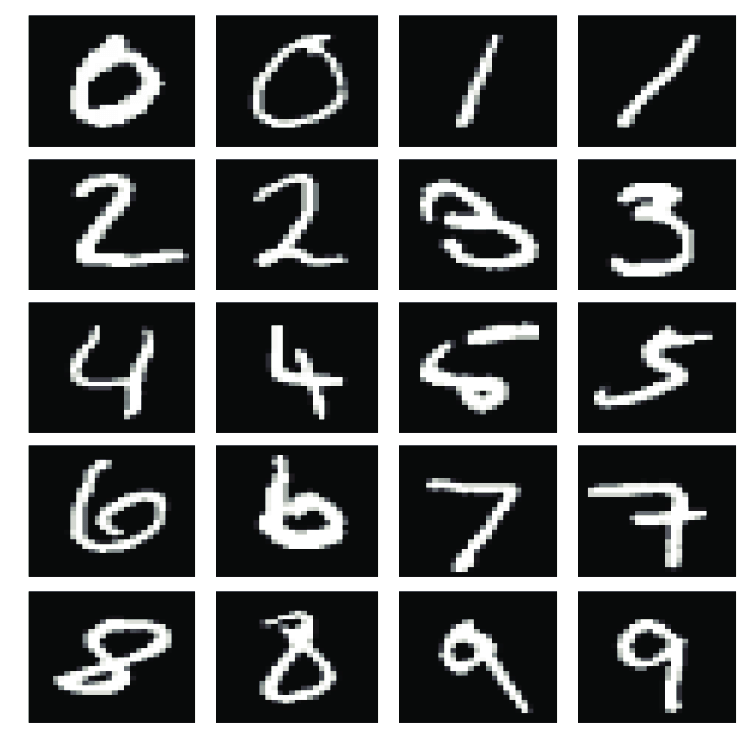
\includegraphics[scale=0.13]{source/mnist.png}
\end{center}
\end{block}
\end{frame}

\section{Linear algebra background}

\begin{frame} {least norm solution}
\begin{block}{normal equation}
problem: \(\min \frac{1}{2} x^Tx \text{ s.t. } Ax = b\) with \(A\) ¸full row rank
\pause
\begin{align*}
	L(x,\lambda) &= \frac{1}{2} x^Tx - \lambda^T (Ax -b)\\
	\nabla_x L(x,\lambda) &= x - A^T \lambda \stackrel{!}{=} 0\\
	x & = A^T \lambda\\
	AA^T \lambda &= b \Leftrightarrow \lambda = (AA^T)^{-1} b\\
	x &= A^T(AA^T)^{-1} b & A^T =: QR\\
	x &= QR(R^TQ^TQR)^{-1}b\\
	x &= QRR^{-1} R^{-T}b\\
	x &= QR^{-T}b
\end{align*}
\end{block}
\end{frame}

\begin{frame}{least squares solution}
\begin{block}{QR decomposition}
\begin{align*}
	A^TAx &= A^T b & \text{normal equation}\\
	R^TQ^TQR^Tx &= R^TQ^Tb\\
	R^TRx & = R^TQ^Tb\\
	Rx &= Q^T b\\
\end{align*}
\end{block}
\end{frame}

\section{Benign Overfitting}

\begin{frame}{polynomial fitting}
\begin{block}{unregulated  estimation of \(\theta\)}
given samples \((x_1, y_1), ..., (x_n, y_n)\)

		\begin{equation*}
			X^T = \begin{pmatrix}
			1 & x_1 & ... & x_1^{k-1}\\
			\vdots &&& \vdots\\
			1 & x_n & ... & x_n^{k-1}
			\end{pmatrix} \text{Vandermondematrix}
		\end{equation*}
		
compute \(\theta\) as least square solution of

\begin{equation}
X^T \theta = y
\end{equation}
\end{block}
\end{frame}

\begin{frame}{polynomial fitting}
\begin{block}{regularized estimation of \(\theta\)}
	problem: \(\min \frac{1}{2} \norm{X^T  \theta -y}^2 + \mu x^TWx\)
	\vspace{0.5cm}
	\pause
	
	\(\mu\) - weight of regularization term
	
	\(W\) - diagonal matrix, \(w_{ij} := \delta_{ij} i \quad i,j \in \{0,...,k-1\}\)
\end{block}
\end{frame}

\begin{frame}{polynomial fitting examples}
\begin{center}
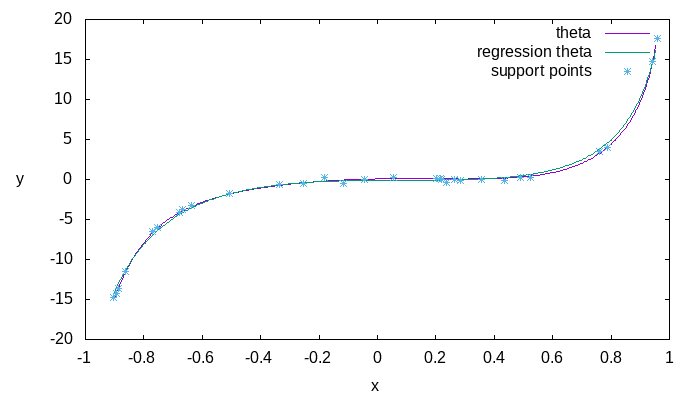
\includegraphics[scale=0.6]{source/theta_plot_1.png}
\end{center}
\end{frame}

\begin{frame}{polynomial fitting examples}
\begin{center}
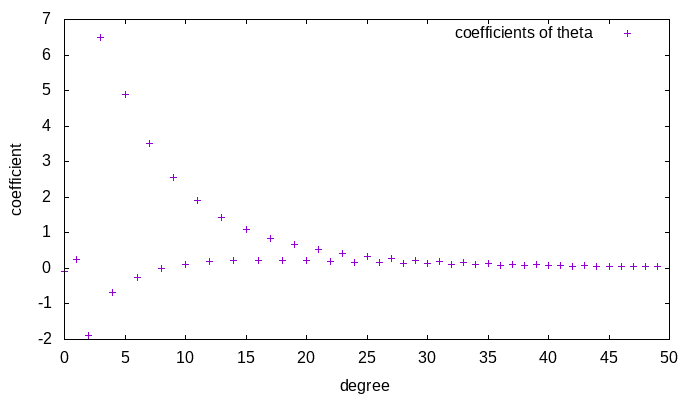
\includegraphics[scale=0.6]{source/theta_coefficients_1.png}
\end{center}
\end{frame}

\begin{frame}{polynomial fitting examples}
\begin{center}
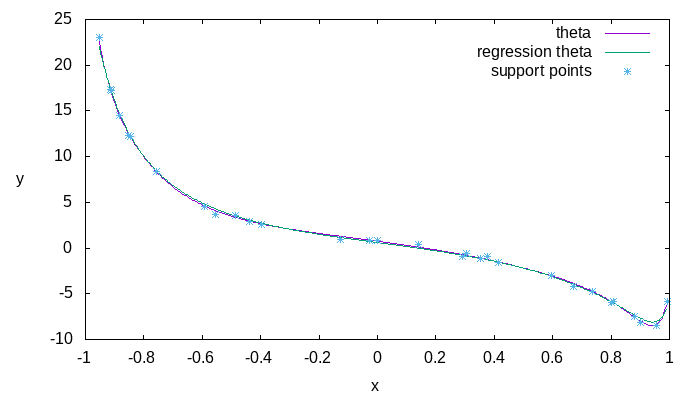
\includegraphics[scale=0.6]{source/theta_plot_2.png}
\end{center}
\end{frame}

\begin{frame}{polynomial fitting examples}
\begin{center}
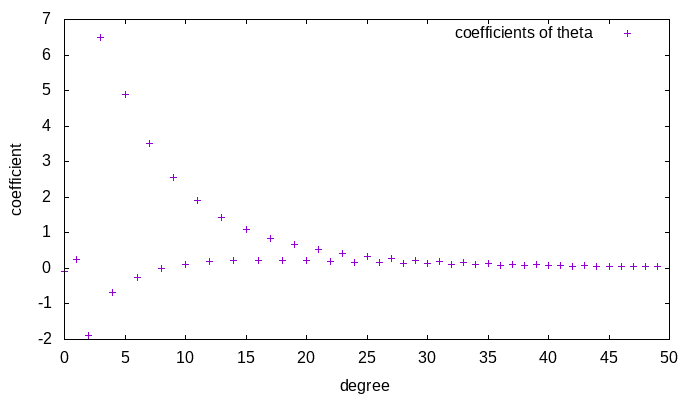
\includegraphics[scale=0.6]{source/theta_coefficients_1.png}
\end{center}
\end{frame}


\section{Sources}
\begin{frame}{Sources}
\begin{block}{Text}
\tiny
\url{http://yann.lecun.com/exdb/mnist/} 13.09.2021 21:45
\end{block}
\end{frame}

\begin{frame}{Sources}
\begin{block}{Images}
\tiny
\begin{itemize}
	\item \url{https://www.researchgate.net/figure/Some-images-in-MNIST-dataset-The-whole-dataset-contains-70-000-2828-gray-scale-images_fig2_330700481} - 11.09.2021 9:58
\end{itemize}
\end{block}
\end{frame}
\end{document}